\subsection{Join network \rom{2}}

\begin{figure}[htb!]
  \centering
    \subfloat[]{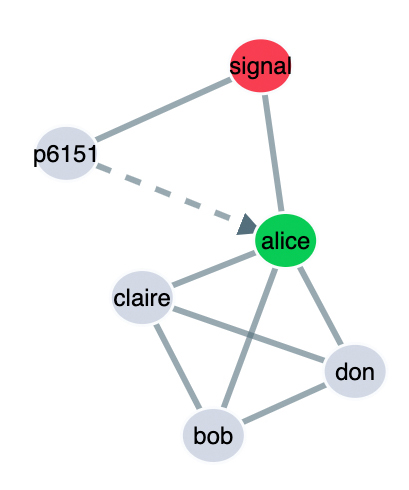
\includegraphics[width=0.33\textwidth]{graphics/analysis/mini-scenarios/router-full-redirect/1.jpg} \label{fig:filmstrips-redirect-a}}
    \subfloat[]{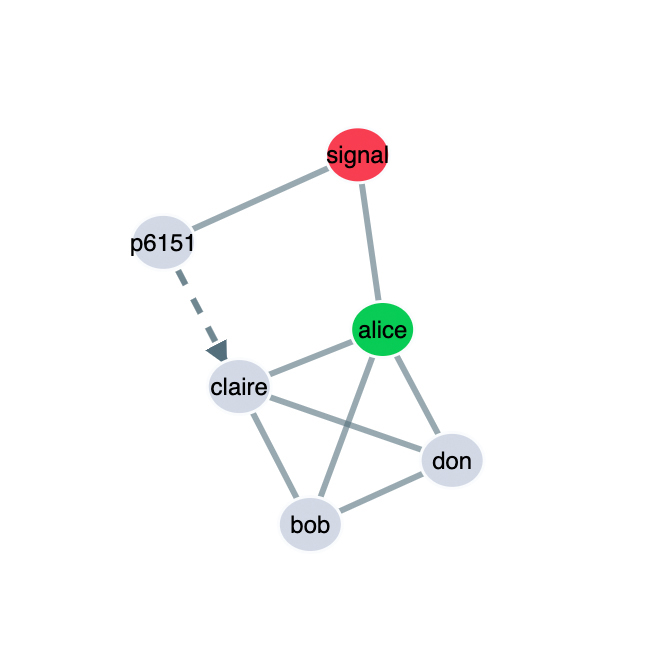
\includegraphics[width=0.33\textwidth]{graphics/analysis/mini-scenarios/router-full-redirect/2.jpg} \label{fig:filmstrips-redirect-b}}
	\subfloat[]{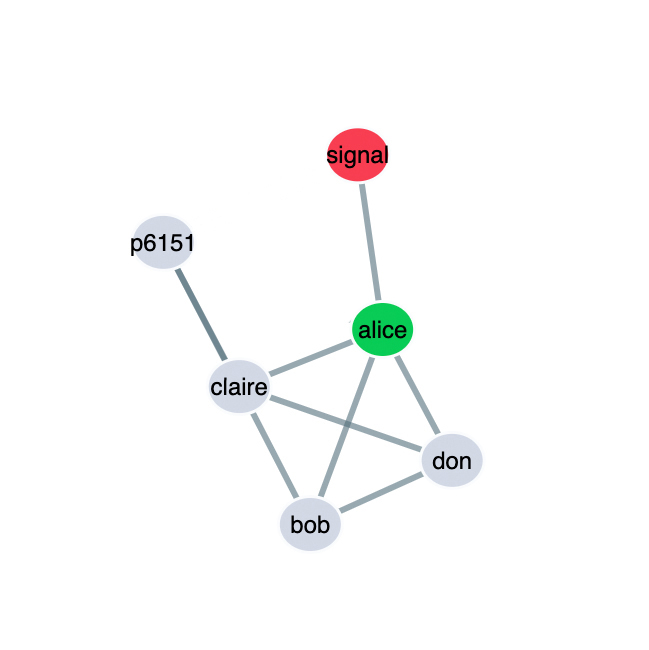
\includegraphics[width=0.33\textwidth]{graphics/analysis/mini-scenarios/router-full-redirect/3.jpg} \label{fig:filmstrips-redirect-c}}
	\caption{Join network, router has no capacity}
\label{fig:filmstrips-redirect}
\end{figure}

A new peer is joining the network, therefor it tries to establish a connection to the \router peer \alice by sending her a connection offer \vref{fig:filmstrips-redirect-a}. 
Yet, \alice has already reached the maximum of connections, that has been configured for this scenario to $\ 4 $. Thus, \alice is rejecting the offer but is also sending a selection of known peer as \textit{Peer-Suggestions}.

The new peer updates its table with the suggestions of \alice. To satisfy the connection goal it sends connection offers to the suggested peer. In this case it sends a connection offer to \claire. The offer is transmitted via \signal and \alice (\vref{fig:filmstrips-redirect-b}). 

\claire receives the offer and as she has one connection available she is sending back her answer to the new peer. The answer is transmitted via \alice and \signal. As soon as the new peer receives the answer, its establishes the connection (\vref{fig:filmstrips-redirect-c}).
